% Created by tikzDevice version 0.12.3.1 on 2023-05-10 22:57:12
% !TEX encoding = UTF-8 Unicode
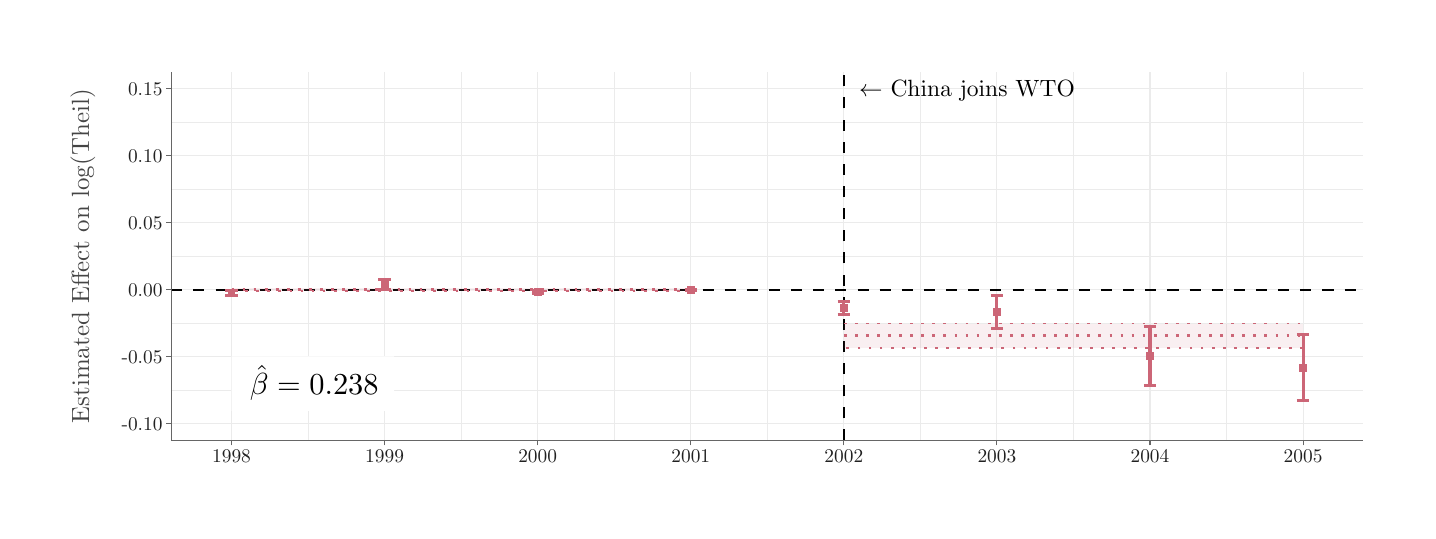
\begin{tikzpicture}[x=1pt,y=1pt]
\definecolor{fillColor}{RGB}{255,255,255}
\path[use as bounding box,fill=fillColor,fill opacity=0.00] (0,0) rectangle (498.66,174.53);
\begin{scope}
\path[clip] (  0.00,  0.00) rectangle (498.66,174.53);
\definecolor{fillColor}{RGB}{255,255,255}

\path[fill=fillColor] (  0.00,  0.00) rectangle (498.66,174.53);
\end{scope}
\begin{scope}
\path[clip] ( 51.87, 25.33) rectangle (482.66,158.53);
\definecolor{fillColor}{RGB}{255,255,255}

\path[fill=fillColor] ( 51.87, 25.33) rectangle (482.66,158.53);
\definecolor{drawColor}{gray}{0.92}

\path[draw=drawColor,line width= 0.2pt,line join=round] ( 51.87, 43.50) --
	(482.66, 43.50);

\path[draw=drawColor,line width= 0.2pt,line join=round] ( 51.87, 67.71) --
	(482.66, 67.71);

\path[draw=drawColor,line width= 0.2pt,line join=round] ( 51.87, 91.93) --
	(482.66, 91.93);

\path[draw=drawColor,line width= 0.2pt,line join=round] ( 51.87,116.15) --
	(482.66,116.15);

\path[draw=drawColor,line width= 0.2pt,line join=round] ( 51.87,140.37) --
	(482.66,140.37);

\path[draw=drawColor,line width= 0.2pt,line join=round] (101.32, 25.33) --
	(101.32,158.53);

\path[draw=drawColor,line width= 0.2pt,line join=round] (156.63, 25.33) --
	(156.63,158.53);

\path[draw=drawColor,line width= 0.2pt,line join=round] (211.95, 25.33) --
	(211.95,158.53);

\path[draw=drawColor,line width= 0.2pt,line join=round] (267.27, 25.33) --
	(267.27,158.53);

\path[draw=drawColor,line width= 0.2pt,line join=round] (322.58, 25.33) --
	(322.58,158.53);

\path[draw=drawColor,line width= 0.2pt,line join=round] (377.90, 25.33) --
	(377.90,158.53);

\path[draw=drawColor,line width= 0.2pt,line join=round] (433.21, 25.33) --
	(433.21,158.53);

\path[draw=drawColor,line width= 0.4pt,line join=round] ( 51.87, 31.39) --
	(482.66, 31.39);

\path[draw=drawColor,line width= 0.4pt,line join=round] ( 51.87, 55.60) --
	(482.66, 55.60);

\path[draw=drawColor,line width= 0.4pt,line join=round] ( 51.87, 79.82) --
	(482.66, 79.82);

\path[draw=drawColor,line width= 0.4pt,line join=round] ( 51.87,104.04) --
	(482.66,104.04);

\path[draw=drawColor,line width= 0.4pt,line join=round] ( 51.87,128.26) --
	(482.66,128.26);

\path[draw=drawColor,line width= 0.4pt,line join=round] ( 51.87,152.48) --
	(482.66,152.48);

\path[draw=drawColor,line width= 0.4pt,line join=round] ( 73.66, 25.33) --
	( 73.66,158.53);

\path[draw=drawColor,line width= 0.4pt,line join=round] (128.98, 25.33) --
	(128.98,158.53);

\path[draw=drawColor,line width= 0.4pt,line join=round] (184.29, 25.33) --
	(184.29,158.53);

\path[draw=drawColor,line width= 0.4pt,line join=round] (239.61, 25.33) --
	(239.61,158.53);

\path[draw=drawColor,line width= 0.4pt,line join=round] (294.92, 25.33) --
	(294.92,158.53);

\path[draw=drawColor,line width= 0.4pt,line join=round] (350.24, 25.33) --
	(350.24,158.53);

\path[draw=drawColor,line width= 0.4pt,line join=round] (405.55, 25.33) --
	(405.55,158.53);

\path[draw=drawColor,line width= 0.4pt,line join=round] (460.87, 25.33) --
	(460.87,158.53);
\definecolor{drawColor}{RGB}{0,0,0}

\path[draw=drawColor,line width= 0.6pt,dash pattern=on 4pt off 4pt ,line join=round] ( 51.87, 79.82) -- (482.66, 79.82);

\path[draw=drawColor,line width= 0.6pt,dash pattern=on 4pt off 4pt ,line join=round] (294.92, 25.33) -- (294.92,158.53);

\node[text=drawColor,anchor=base west,inner sep=0pt, outer sep=0pt, scale=  0.85] at (300.45,149.54) {$\leftarrow$ China joins WTO};

\path[fill=fillColor] ( 73.66, 36.09) --
	(132.40, 36.09) --
	(132.40, 36.09) --
	(132.40, 36.09) --
	(132.40, 36.09) --
	(132.40, 36.09) --
	(132.40, 36.09) --
	(132.40, 36.09) --
	(132.40, 36.09) --
	(132.40, 36.09) --
	(132.40, 36.09) --
	(132.40, 36.09) --
	(132.40, 36.09) --
	(132.40, 36.09) --
	(132.40, 55.74) --
	(132.40, 55.74) --
	(132.40, 55.74) --
	(132.40, 55.74) --
	(132.40, 55.74) --
	(132.40, 55.74) --
	(132.40, 55.74) --
	(132.40, 55.74) --
	(132.40, 55.74) --
	(132.40, 55.74) --
	(132.40, 55.74) --
	(132.40, 55.74) --
	( 73.66, 55.74) --
	( 73.66, 55.74) --
	( 73.66, 55.74) --
	( 73.66, 55.74) --
	( 73.66, 55.74) --
	( 73.66, 55.74) --
	( 73.66, 55.74) --
	( 73.66, 55.74) --
	( 73.66, 55.74) --
	( 73.66, 55.74) --
	( 73.66, 55.74) --
	( 73.66, 55.74) --
	( 73.66, 55.74) --
	( 73.66, 36.09) --
	( 73.66, 36.09) --
	( 73.66, 36.09) --
	( 73.66, 36.09) --
	( 73.66, 36.09) --
	( 73.66, 36.09) --
	( 73.66, 36.09) --
	( 73.66, 36.09) --
	( 73.66, 36.09) --
	( 73.66, 36.09) --
	( 73.66, 36.09) --
	( 73.66, 36.09) --
	cycle;
\end{scope}
\begin{scope}
\path[clip] ( 51.87, 25.33) rectangle (482.66,158.53);
\definecolor{drawColor}{RGB}{0,0,0}

\node[text=drawColor,anchor=base west,inner sep=0pt, outer sep=0pt, scale=  1.10] at ( 80.31, 42.12) {$\hat{\beta} = 0.238$};
\definecolor{drawColor}{RGB}{204,102,119}

\path[draw=drawColor,line width= 1.1pt,line join=round] ( 71.45, 79.67) --
	( 75.87, 79.67);

\path[draw=drawColor,line width= 1.1pt,line join=round] ( 73.66, 79.67) --
	( 73.66, 77.85);

\path[draw=drawColor,line width= 1.1pt,line join=round] ( 71.45, 77.85) --
	( 75.87, 77.85);

\path[draw=drawColor,line width= 1.1pt,line join=round] (126.76, 83.38) --
	(131.19, 83.38);

\path[draw=drawColor,line width= 1.1pt,line join=round] (128.98, 83.38) --
	(128.98, 80.09);

\path[draw=drawColor,line width= 1.1pt,line join=round] (126.76, 80.09) --
	(131.19, 80.09);

\path[draw=drawColor,line width= 1.1pt,line join=round] (182.08, 79.72) --
	(186.51, 79.72);

\path[draw=drawColor,line width= 1.1pt,line join=round] (184.29, 79.72) --
	(184.29, 78.50);

\path[draw=drawColor,line width= 1.1pt,line join=round] (182.08, 78.50) --
	(186.51, 78.50);

\path[draw=drawColor,line width= 1.1pt,line join=round] (237.40, 79.80) --
	(241.82, 79.80);

\path[draw=drawColor,line width= 1.1pt,line join=round] (239.61, 79.80) --
	(239.61, 79.55);

\path[draw=drawColor,line width= 1.1pt,line join=round] (237.40, 79.55) --
	(241.82, 79.55);

\path[draw=drawColor,line width= 1.1pt,line join=round] (292.71, 75.47) --
	(297.14, 75.47);

\path[draw=drawColor,line width= 1.1pt,line join=round] (294.92, 75.47) --
	(294.92, 70.73);

\path[draw=drawColor,line width= 1.1pt,line join=round] (292.71, 70.73) --
	(297.14, 70.73);

\path[draw=drawColor,line width= 1.1pt,line join=round] (348.03, 77.92) --
	(352.45, 77.92);

\path[draw=drawColor,line width= 1.1pt,line join=round] (350.24, 77.92) --
	(350.24, 65.92);

\path[draw=drawColor,line width= 1.1pt,line join=round] (348.03, 65.92) --
	(352.45, 65.92);

\path[draw=drawColor,line width= 1.1pt,line join=round] (403.34, 66.69) --
	(407.77, 66.69);

\path[draw=drawColor,line width= 1.1pt,line join=round] (405.55, 66.69) --
	(405.55, 45.14);

\path[draw=drawColor,line width= 1.1pt,line join=round] (403.34, 45.14) --
	(407.77, 45.14);

\path[draw=drawColor,line width= 1.1pt,line join=round] (458.66, 63.76) --
	(463.08, 63.76);

\path[draw=drawColor,line width= 1.1pt,line join=round] (460.87, 63.76) --
	(460.87, 39.64);

\path[draw=drawColor,line width= 1.1pt,line join=round] (458.66, 39.64) --
	(463.08, 39.64);
\definecolor{fillColor}{RGB}{204,102,119}

\path[fill=fillColor] ( 72.24, 77.34) --
	( 75.09, 77.34) --
	( 75.09, 80.19) --
	( 72.24, 80.19) --
	cycle;

\path[fill=fillColor] (127.55, 80.31) --
	(130.40, 80.31) --
	(130.40, 83.16) --
	(127.55, 83.16) --
	cycle;

\path[fill=fillColor] (182.87, 77.69) --
	(185.72, 77.69) --
	(185.72, 80.54) --
	(182.87, 80.54) --
	cycle;

\path[fill=fillColor] (238.18, 78.25) --
	(241.03, 78.25) --
	(241.03, 81.11) --
	(238.18, 81.11) --
	cycle;

\path[fill=fillColor] (293.50, 71.67) --
	(296.35, 71.67) --
	(296.35, 74.52) --
	(293.50, 74.52) --
	cycle;

\path[fill=fillColor] (348.81, 70.49) --
	(351.66, 70.49) --
	(351.66, 73.34) --
	(348.81, 73.34) --
	cycle;

\path[fill=fillColor] (404.13, 54.49) --
	(406.98, 54.49) --
	(406.98, 57.34) --
	(404.13, 57.34) --
	cycle;

\path[fill=fillColor] (459.44, 50.27) --
	(462.30, 50.27) --
	(462.30, 53.13) --
	(459.44, 53.13) --
	cycle;
\definecolor{fillColor}{RGB}{204,102,119}

\path[fill=fillColor,fill opacity=0.10] (294.92, 67.62) --
	(460.87, 67.62) --
	(460.87, 58.69) --
	(294.92, 58.69) --
	cycle;

\path[draw=drawColor,line width= 0.6pt,dash pattern=on 1pt off 3pt ,line join=round] (294.92, 67.62) --
	(460.87, 67.62);

\path[draw=drawColor,line width= 0.6pt,dash pattern=on 1pt off 3pt ,line join=round] (460.87, 58.69) --
	(294.92, 58.69);

\path[fill=fillColor,fill opacity=0.10] ( 73.66, 80.33) --
	(239.61, 80.33) --
	(239.61, 79.31) --
	( 73.66, 79.31) --
	cycle;

\path[draw=drawColor,line width= 0.6pt,dash pattern=on 1pt off 3pt ,line join=round] ( 73.66, 80.33) --
	(239.61, 80.33);

\path[draw=drawColor,line width= 0.6pt,dash pattern=on 1pt off 3pt ,line join=round] (239.61, 79.31) --
	( 73.66, 79.31);

\path[draw=drawColor,line width= 1.1pt,dash pattern=on 1pt off 3pt ,line join=round] (294.92, 63.16) --
	(460.87, 63.16);

\path[draw=drawColor,line width= 1.1pt,dash pattern=on 1pt off 3pt ,line join=round] ( 73.66, 79.82) --
	(239.61, 79.82);
\end{scope}
\begin{scope}
\path[clip] (  0.00,  0.00) rectangle (498.66,174.53);
\definecolor{drawColor}{gray}{0.40}

\path[draw=drawColor,line width= 0.4pt,line join=round] ( 51.87, 25.33) --
	( 51.87,158.53);
\end{scope}
\begin{scope}
\path[clip] (  0.00,  0.00) rectangle (498.66,174.53);
\definecolor{drawColor}{gray}{0.13}

\node[text=drawColor,anchor=base east,inner sep=0pt, outer sep=0pt, scale=  0.70] at ( 48.72, 28.98) {-0.10};

\node[text=drawColor,anchor=base east,inner sep=0pt, outer sep=0pt, scale=  0.70] at ( 48.72, 53.19) {-0.05};

\node[text=drawColor,anchor=base east,inner sep=0pt, outer sep=0pt, scale=  0.70] at ( 48.72, 77.41) {0.00};

\node[text=drawColor,anchor=base east,inner sep=0pt, outer sep=0pt, scale=  0.70] at ( 48.72,101.63) {0.05};

\node[text=drawColor,anchor=base east,inner sep=0pt, outer sep=0pt, scale=  0.70] at ( 48.72,125.85) {0.10};

\node[text=drawColor,anchor=base east,inner sep=0pt, outer sep=0pt, scale=  0.70] at ( 48.72,150.07) {0.15};
\end{scope}
\begin{scope}
\path[clip] (  0.00,  0.00) rectangle (498.66,174.53);
\definecolor{drawColor}{gray}{0.40}

\path[draw=drawColor,line width= 0.4pt,line join=round] ( 50.12, 31.39) --
	( 51.87, 31.39);

\path[draw=drawColor,line width= 0.4pt,line join=round] ( 50.12, 55.60) --
	( 51.87, 55.60);

\path[draw=drawColor,line width= 0.4pt,line join=round] ( 50.12, 79.82) --
	( 51.87, 79.82);

\path[draw=drawColor,line width= 0.4pt,line join=round] ( 50.12,104.04) --
	( 51.87,104.04);

\path[draw=drawColor,line width= 0.4pt,line join=round] ( 50.12,128.26) --
	( 51.87,128.26);

\path[draw=drawColor,line width= 0.4pt,line join=round] ( 50.12,152.48) --
	( 51.87,152.48);
\end{scope}
\begin{scope}
\path[clip] (  0.00,  0.00) rectangle (498.66,174.53);
\definecolor{drawColor}{gray}{0.40}

\path[draw=drawColor,line width= 0.4pt,line join=round] ( 51.87, 25.33) --
	(482.66, 25.33);
\end{scope}
\begin{scope}
\path[clip] (  0.00,  0.00) rectangle (498.66,174.53);
\definecolor{drawColor}{gray}{0.40}

\path[draw=drawColor,line width= 0.4pt,line join=round] ( 73.66, 23.58) --
	( 73.66, 25.33);

\path[draw=drawColor,line width= 0.4pt,line join=round] (128.98, 23.58) --
	(128.98, 25.33);

\path[draw=drawColor,line width= 0.4pt,line join=round] (184.29, 23.58) --
	(184.29, 25.33);

\path[draw=drawColor,line width= 0.4pt,line join=round] (239.61, 23.58) --
	(239.61, 25.33);

\path[draw=drawColor,line width= 0.4pt,line join=round] (294.92, 23.58) --
	(294.92, 25.33);

\path[draw=drawColor,line width= 0.4pt,line join=round] (350.24, 23.58) --
	(350.24, 25.33);

\path[draw=drawColor,line width= 0.4pt,line join=round] (405.55, 23.58) --
	(405.55, 25.33);

\path[draw=drawColor,line width= 0.4pt,line join=round] (460.87, 23.58) --
	(460.87, 25.33);
\end{scope}
\begin{scope}
\path[clip] (  0.00,  0.00) rectangle (498.66,174.53);
\definecolor{drawColor}{gray}{0.13}

\node[text=drawColor,anchor=base,inner sep=0pt, outer sep=0pt, scale=  0.70] at ( 73.66, 17.36) {1998};

\node[text=drawColor,anchor=base,inner sep=0pt, outer sep=0pt, scale=  0.70] at (128.98, 17.36) {1999};

\node[text=drawColor,anchor=base,inner sep=0pt, outer sep=0pt, scale=  0.70] at (184.29, 17.36) {2000};

\node[text=drawColor,anchor=base,inner sep=0pt, outer sep=0pt, scale=  0.70] at (239.61, 17.36) {2001};

\node[text=drawColor,anchor=base,inner sep=0pt, outer sep=0pt, scale=  0.70] at (294.92, 17.36) {2002};

\node[text=drawColor,anchor=base,inner sep=0pt, outer sep=0pt, scale=  0.70] at (350.24, 17.36) {2003};

\node[text=drawColor,anchor=base,inner sep=0pt, outer sep=0pt, scale=  0.70] at (405.55, 17.36) {2004};

\node[text=drawColor,anchor=base,inner sep=0pt, outer sep=0pt, scale=  0.70] at (460.87, 17.36) {2005};
\end{scope}
\begin{scope}
\path[clip] (  0.00,  0.00) rectangle (498.66,174.53);
\definecolor{drawColor}{gray}{0.27}

\node[text=drawColor,rotate= 90.00,anchor=base,inner sep=0pt, outer sep=0pt, scale=  0.90] at ( 22.20, 91.93) {Estimated Effect on $\log($Theil$)$};
\end{scope}
\end{tikzpicture}
